\documentclass[twoside]{book}

% Packages required by doxygen
\usepackage{fixltx2e}
\usepackage{calc}
\usepackage{doxygen}
\usepackage[export]{adjustbox} % also loads graphicx
\usepackage{graphicx}
\usepackage[utf8]{inputenc}
\usepackage{makeidx}
\usepackage{multicol}
\usepackage{multirow}
\PassOptionsToPackage{warn}{textcomp}
\usepackage{textcomp}
\usepackage[nointegrals]{wasysym}
\usepackage[table]{xcolor}

% Font selection
\usepackage[T1]{fontenc}
\usepackage[scaled=.90]{helvet}
\usepackage{courier}
\usepackage{amssymb}
\usepackage{sectsty}
\renewcommand{\familydefault}{\sfdefault}
\allsectionsfont{%
  \fontseries{bc}\selectfont%
  \color{darkgray}%
}
\renewcommand{\DoxyLabelFont}{%
  \fontseries{bc}\selectfont%
  \color{darkgray}%
}
\newcommand{\+}{\discretionary{\mbox{\scriptsize$\hookleftarrow$}}{}{}}

% Page & text layout
\usepackage{geometry}
\geometry{%
  a4paper,%
  top=2.5cm,%
  bottom=2.5cm,%
  left=2.5cm,%
  right=2.5cm%
}
\tolerance=750
\hfuzz=15pt
\hbadness=750
\setlength{\emergencystretch}{15pt}
\setlength{\parindent}{0cm}
\setlength{\parskip}{3ex plus 2ex minus 2ex}
\makeatletter
\renewcommand{\paragraph}{%
  \@startsection{paragraph}{4}{0ex}{-1.0ex}{1.0ex}{%
    \normalfont\normalsize\bfseries\SS@parafont%
  }%
}
\renewcommand{\subparagraph}{%
  \@startsection{subparagraph}{5}{0ex}{-1.0ex}{1.0ex}{%
    \normalfont\normalsize\bfseries\SS@subparafont%
  }%
}
\makeatother

% Headers & footers
\usepackage{fancyhdr}
\pagestyle{fancyplain}
\fancyhead[LE]{\fancyplain{}{\bfseries\thepage}}
\fancyhead[CE]{\fancyplain{}{}}
\fancyhead[RE]{\fancyplain{}{\bfseries\leftmark}}
\fancyhead[LO]{\fancyplain{}{\bfseries\rightmark}}
\fancyhead[CO]{\fancyplain{}{}}
\fancyhead[RO]{\fancyplain{}{\bfseries\thepage}}
\fancyfoot[LE]{\fancyplain{}{}}
\fancyfoot[CE]{\fancyplain{}{}}
\fancyfoot[RE]{\fancyplain{}{\bfseries\scriptsize Generated by Doxygen }}
\fancyfoot[LO]{\fancyplain{}{\bfseries\scriptsize Generated by Doxygen }}
\fancyfoot[CO]{\fancyplain{}{}}
\fancyfoot[RO]{\fancyplain{}{}}
\renewcommand{\footrulewidth}{0.4pt}
\renewcommand{\chaptermark}[1]{%
  \markboth{#1}{}%
}
\renewcommand{\sectionmark}[1]{%
  \markright{\thesection\ #1}%
}

% Indices & bibliography
\usepackage{natbib}
\usepackage[titles]{tocloft}
\setcounter{tocdepth}{3}
\setcounter{secnumdepth}{5}
\makeindex

% Hyperlinks (required, but should be loaded last)
\usepackage{ifpdf}
\ifpdf
  \usepackage[pdftex,pagebackref=true]{hyperref}
\else
  \usepackage[ps2pdf,pagebackref=true]{hyperref}
\fi
\hypersetup{%
  colorlinks=true,%
  linkcolor=blue,%
  citecolor=blue,%
  unicode%
}

% Custom commands
\newcommand{\clearemptydoublepage}{%
  \newpage{\pagestyle{empty}\cleardoublepage}%
}

\usepackage{caption}
\captionsetup{labelsep=space,justification=centering,font={bf},singlelinecheck=off,skip=4pt,position=top}

%===== C O N T E N T S =====

\begin{document}

% Titlepage & ToC
\hypersetup{pageanchor=false,
             bookmarksnumbered=true,
             pdfencoding=unicode
            }
\pagenumbering{alph}
\begin{titlepage}
\vspace*{7cm}
\begin{center}%
{\Large Elevator\+\_\+project }\\
\vspace*{1cm}
{\large Generated by Doxygen 1.8.13}\\
\end{center}
\end{titlepage}
\clearemptydoublepage
\pagenumbering{roman}
\tableofcontents
\clearemptydoublepage
\pagenumbering{arabic}
\hypersetup{pageanchor=true}

%--- Begin generated contents ---
\chapter{File Index}
\section{File List}
Here is a list of all documented files with brief descriptions\+:\begin{DoxyCompactList}
\item\contentsline{section}{source/\hyperlink{hardware_8h}{hardware.\+h} \\*Driver for the elevator hardware }{\pageref{hardware_8h}}{}
\item\contentsline{section}{source/{\bfseries lights.\+c} }{\pageref{lights_8c}}{}
\item\contentsline{section}{source/\hyperlink{lights_8h}{lights.\+h} \\*A library for doing operations on the lights on the floor-\/panel }{\pageref{lights_8h}}{}
\item\contentsline{section}{source/{\bfseries main.\+c} }{\pageref{main_8c}}{}
\item\contentsline{section}{source/{\bfseries orders.\+c} }{\pageref{orders_8c}}{}
\item\contentsline{section}{source/\hyperlink{orders_8h}{orders.\+h} \\*Implementation of management of orders }{\pageref{orders_8h}}{}
\item\contentsline{section}{source/{\bfseries queue.\+c} }{\pageref{queue_8c}}{}
\item\contentsline{section}{source/\hyperlink{queue_8h}{queue.\+h} \\*Library for the implementation of queue }{\pageref{queue_8h}}{}
\item\contentsline{section}{source/{\bfseries state.\+c} }{\pageref{state_8c}}{}
\item\contentsline{section}{source/\hyperlink{state_8h}{state.\+h} \\*Library for the implementation of the State Machine }{\pageref{state_8h}}{}
\item\contentsline{section}{source/{\bfseries timer.\+c} }{\pageref{timer_8c}}{}
\item\contentsline{section}{source/\hyperlink{timer_8h}{timer.\+h} \\*Implementation of timer on the elevator door }{\pageref{timer_8h}}{}
\end{DoxyCompactList}

\chapter{File Documentation}
\hypertarget{hardware_8h}{}\section{source/hardware.h File Reference}
\label{hardware_8h}\index{source/hardware.\+h@{source/hardware.\+h}}


Driver for the elevator hardware.  


This graph shows which files directly or indirectly include this file\+:
\nopagebreak
\begin{figure}[H]
\begin{center}
\leavevmode
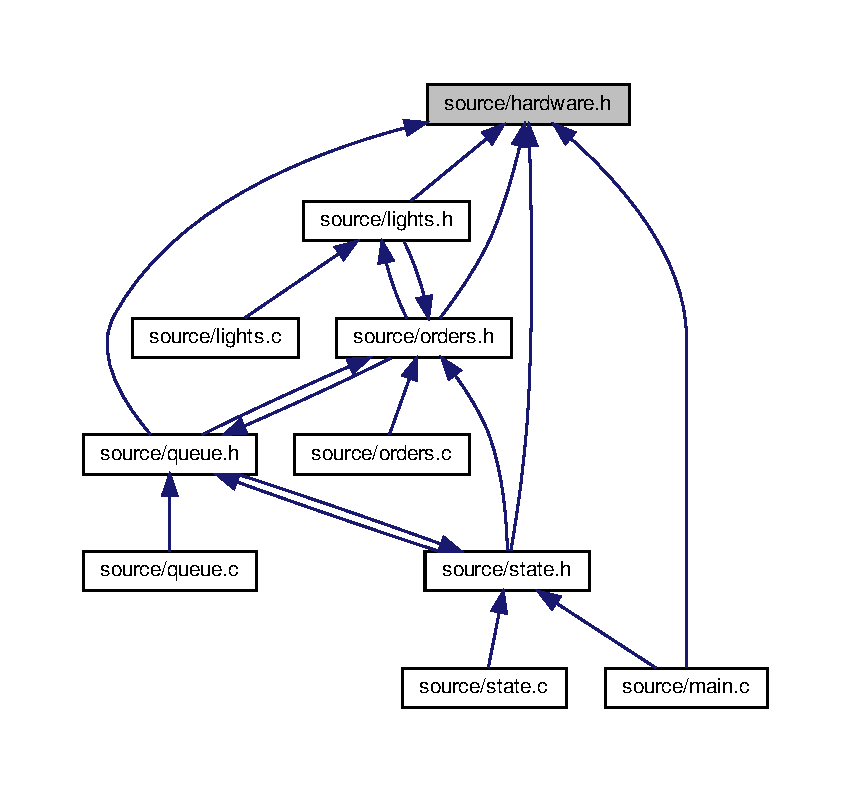
\includegraphics[width=350pt]{hardware_8h__dep__incl}
\end{center}
\end{figure}
\subsection*{Macros}
\begin{DoxyCompactItemize}
\item 
\mbox{\Hypertarget{hardware_8h_ae9e42615eade15633bd8c03b7a271a00}\label{hardware_8h_ae9e42615eade15633bd8c03b7a271a00}} 
\#define {\bfseries H\+A\+R\+D\+W\+A\+R\+E\+\_\+\+N\+U\+M\+B\+E\+R\+\_\+\+O\+F\+\_\+\+F\+L\+O\+O\+RS}~4
\item 
\mbox{\Hypertarget{hardware_8h_a966cbacea011640db5803364bff5ed53}\label{hardware_8h_a966cbacea011640db5803364bff5ed53}} 
\#define {\bfseries H\+A\+R\+D\+W\+A\+R\+E\+\_\+\+N\+U\+M\+B\+E\+R\+\_\+\+O\+F\+\_\+\+B\+U\+T\+T\+O\+NS}~3
\end{DoxyCompactItemize}
\subsection*{Enumerations}
\begin{DoxyCompactItemize}
\item 
\mbox{\Hypertarget{hardware_8h_a2167c399a24df296afc432bcb88228af}\label{hardware_8h_a2167c399a24df296afc432bcb88228af}} 
enum \hyperlink{hardware_8h_a2167c399a24df296afc432bcb88228af}{Hardware\+Movement} \{ {\bfseries H\+A\+R\+D\+W\+A\+R\+E\+\_\+\+M\+O\+V\+E\+M\+E\+N\+T\+\_\+\+UP}, 
{\bfseries H\+A\+R\+D\+W\+A\+R\+E\+\_\+\+M\+O\+V\+E\+M\+E\+N\+T\+\_\+\+S\+T\+OP}, 
{\bfseries H\+A\+R\+D\+W\+A\+R\+E\+\_\+\+M\+O\+V\+E\+M\+E\+N\+T\+\_\+\+D\+O\+WN}
 \}\begin{DoxyCompactList}\small\item\em Movement type used in {\ttfamily hardware\+\_\+command\+\_\+movement}. \end{DoxyCompactList}
\item 
\mbox{\Hypertarget{hardware_8h_a796a8de8ce0ae769d7dbd3327a7bdbe7}\label{hardware_8h_a796a8de8ce0ae769d7dbd3327a7bdbe7}} 
enum \hyperlink{hardware_8h_a796a8de8ce0ae769d7dbd3327a7bdbe7}{Hardware\+Order} \{ {\bfseries H\+A\+R\+D\+W\+A\+R\+E\+\_\+\+O\+R\+D\+E\+R\+\_\+\+UP}, 
{\bfseries H\+A\+R\+D\+W\+A\+R\+E\+\_\+\+O\+R\+D\+E\+R\+\_\+\+I\+N\+S\+I\+DE}, 
{\bfseries H\+A\+R\+D\+W\+A\+R\+E\+\_\+\+O\+R\+D\+E\+R\+\_\+\+D\+O\+WN}
 \}\begin{DoxyCompactList}\small\item\em Order type used in {\ttfamily hardware\+\_\+read\+\_\+order} and in {\ttfamily hardware\+\_\+command\+\_\+order\+\_\+light}. \end{DoxyCompactList}
\end{DoxyCompactItemize}
\subsection*{Functions}
\begin{DoxyCompactItemize}
\item 
int \hyperlink{hardware_8h_a054b8fb8768311d46be58d6a4890d771}{hardware\+\_\+init} ()
\begin{DoxyCompactList}\small\item\em Initializes the elevator control hardware. Must be called once before other calls to the elevator hardware driver. \end{DoxyCompactList}\item 
void \hyperlink{hardware_8h_a01de081ef0510a111053c18cd31afa27}{hardware\+\_\+command\+\_\+movement} (\hyperlink{hardware_8h_a2167c399a24df296afc432bcb88228af}{Hardware\+Movement} movement)
\begin{DoxyCompactList}\small\item\em Commands the elevator to either move up or down, or commands it to halt. \end{DoxyCompactList}\item 
int \hyperlink{hardware_8h_a4a77b27c86675c00b513db3445966804}{hardware\+\_\+read\+\_\+stop\+\_\+signal} ()
\begin{DoxyCompactList}\small\item\em Polls the hardware for the current stop signal. \end{DoxyCompactList}\item 
int \hyperlink{hardware_8h_a459fe57a3ee4bc2a28e8a15b2ab14c2d}{hardware\+\_\+read\+\_\+obstruction\+\_\+signal} ()
\begin{DoxyCompactList}\small\item\em Polls the hardware for the current obstruction signal. \end{DoxyCompactList}\item 
int \hyperlink{hardware_8h_ab048489e6302bb5604aad753f2d7d501}{hardware\+\_\+read\+\_\+floor\+\_\+sensor} (int floor)
\begin{DoxyCompactList}\small\item\em Polls the floor sensor for the given {\ttfamily floor}. \end{DoxyCompactList}\item 
int \hyperlink{hardware_8h_a87917f3aa093fb46ca821a400d011ee8}{hardware\+\_\+read\+\_\+order} (int floor, \hyperlink{hardware_8h_a796a8de8ce0ae769d7dbd3327a7bdbe7}{Hardware\+Order} order\+\_\+type)
\begin{DoxyCompactList}\small\item\em Polls the hardware for the status of orders from floor {\ttfamily floor} of type {\ttfamily order\+\_\+type}. \end{DoxyCompactList}\item 
void \hyperlink{hardware_8h_a80d99ddaa8e7b58c9a88b60ea553c1b6}{hardware\+\_\+command\+\_\+door\+\_\+open} (int door\+\_\+open)
\begin{DoxyCompactList}\small\item\em Commands the hardware to open-\/ or close the elevator door. \end{DoxyCompactList}\item 
void \hyperlink{hardware_8h_a407a6ec035ba357de6aa0fbe55501d1e}{hardware\+\_\+command\+\_\+floor\+\_\+indicator\+\_\+on} (int floor)
\begin{DoxyCompactList}\small\item\em Commands the hardware to turn on the floor indicator for {\ttfamily floor}. All indicators all mutually exclusive; other indicator lights will turn off. \end{DoxyCompactList}\item 
void \hyperlink{hardware_8h_aa75b3ac17f72b25946414f48d0063a10}{hardware\+\_\+command\+\_\+stop\+\_\+light} (int on)
\begin{DoxyCompactList}\small\item\em Sets the light in the panel stop button. \end{DoxyCompactList}\item 
void \hyperlink{hardware_8h_aa9b33faa52f0ec5b614d3e7dc05be140}{hardware\+\_\+command\+\_\+order\+\_\+light} (int floor, \hyperlink{hardware_8h_a796a8de8ce0ae769d7dbd3327a7bdbe7}{Hardware\+Order} order\+\_\+type, int on)
\begin{DoxyCompactList}\small\item\em Sets the light in a button corresponding to an order of type {\ttfamily order\+\_\+type}, at floor {\ttfamily floor}. \end{DoxyCompactList}\end{DoxyCompactItemize}


\subsection{Detailed Description}
Driver for the elevator hardware. 



\subsection{Function Documentation}
\mbox{\Hypertarget{hardware_8h_a80d99ddaa8e7b58c9a88b60ea553c1b6}\label{hardware_8h_a80d99ddaa8e7b58c9a88b60ea553c1b6}} 
\index{hardware.\+h@{hardware.\+h}!hardware\+\_\+command\+\_\+door\+\_\+open@{hardware\+\_\+command\+\_\+door\+\_\+open}}
\index{hardware\+\_\+command\+\_\+door\+\_\+open@{hardware\+\_\+command\+\_\+door\+\_\+open}!hardware.\+h@{hardware.\+h}}
\subsubsection{\texorpdfstring{hardware\+\_\+command\+\_\+door\+\_\+open()}{hardware\_command\_door\_open()}}
{\footnotesize\ttfamily void hardware\+\_\+command\+\_\+door\+\_\+open (\begin{DoxyParamCaption}\item[{int}]{door\+\_\+open }\end{DoxyParamCaption})}



Commands the hardware to open-\/ or close the elevator door. 


\begin{DoxyParams}{Parameters}
{\em door\+\_\+open} & A truthy value (non-\/zero) to open the door; 0 to close. \\
\hline
\end{DoxyParams}
\mbox{\Hypertarget{hardware_8h_a407a6ec035ba357de6aa0fbe55501d1e}\label{hardware_8h_a407a6ec035ba357de6aa0fbe55501d1e}} 
\index{hardware.\+h@{hardware.\+h}!hardware\+\_\+command\+\_\+floor\+\_\+indicator\+\_\+on@{hardware\+\_\+command\+\_\+floor\+\_\+indicator\+\_\+on}}
\index{hardware\+\_\+command\+\_\+floor\+\_\+indicator\+\_\+on@{hardware\+\_\+command\+\_\+floor\+\_\+indicator\+\_\+on}!hardware.\+h@{hardware.\+h}}
\subsubsection{\texorpdfstring{hardware\+\_\+command\+\_\+floor\+\_\+indicator\+\_\+on()}{hardware\_command\_floor\_indicator\_on()}}
{\footnotesize\ttfamily void hardware\+\_\+command\+\_\+floor\+\_\+indicator\+\_\+on (\begin{DoxyParamCaption}\item[{int}]{floor }\end{DoxyParamCaption})}



Commands the hardware to turn on the floor indicator for {\ttfamily floor}. All indicators all mutually exclusive; other indicator lights will turn off. 


\begin{DoxyParams}{Parameters}
{\em floor} & Floor to turn on the indicator for.\\
\hline
\end{DoxyParams}
\begin{DoxyWarning}{Warning}
Owing to peculiarities in the hardware construction, there will always be one indicator active. 
\end{DoxyWarning}
\mbox{\Hypertarget{hardware_8h_a01de081ef0510a111053c18cd31afa27}\label{hardware_8h_a01de081ef0510a111053c18cd31afa27}} 
\index{hardware.\+h@{hardware.\+h}!hardware\+\_\+command\+\_\+movement@{hardware\+\_\+command\+\_\+movement}}
\index{hardware\+\_\+command\+\_\+movement@{hardware\+\_\+command\+\_\+movement}!hardware.\+h@{hardware.\+h}}
\subsubsection{\texorpdfstring{hardware\+\_\+command\+\_\+movement()}{hardware\_command\_movement()}}
{\footnotesize\ttfamily void hardware\+\_\+command\+\_\+movement (\begin{DoxyParamCaption}\item[{\hyperlink{hardware_8h_a2167c399a24df296afc432bcb88228af}{Hardware\+Movement}}]{movement }\end{DoxyParamCaption})}



Commands the elevator to either move up or down, or commands it to halt. 


\begin{DoxyParams}{Parameters}
{\em movement} & Commanded movement. \\
\hline
\end{DoxyParams}
\mbox{\Hypertarget{hardware_8h_aa9b33faa52f0ec5b614d3e7dc05be140}\label{hardware_8h_aa9b33faa52f0ec5b614d3e7dc05be140}} 
\index{hardware.\+h@{hardware.\+h}!hardware\+\_\+command\+\_\+order\+\_\+light@{hardware\+\_\+command\+\_\+order\+\_\+light}}
\index{hardware\+\_\+command\+\_\+order\+\_\+light@{hardware\+\_\+command\+\_\+order\+\_\+light}!hardware.\+h@{hardware.\+h}}
\subsubsection{\texorpdfstring{hardware\+\_\+command\+\_\+order\+\_\+light()}{hardware\_command\_order\_light()}}
{\footnotesize\ttfamily void hardware\+\_\+command\+\_\+order\+\_\+light (\begin{DoxyParamCaption}\item[{int}]{floor,  }\item[{\hyperlink{hardware_8h_a796a8de8ce0ae769d7dbd3327a7bdbe7}{Hardware\+Order}}]{order\+\_\+type,  }\item[{int}]{on }\end{DoxyParamCaption})}



Sets the light in a button corresponding to an order of type {\ttfamily order\+\_\+type}, at floor {\ttfamily floor}. 


\begin{DoxyParams}{Parameters}
{\em floor} & The floor of the order indicator. \\
\hline
{\em order\+\_\+type} & The type of order. \\
\hline
{\em on} & A truthy value (non-\/zero) to turn the light on; 0 to turn it off. \\
\hline
\end{DoxyParams}
\mbox{\Hypertarget{hardware_8h_aa75b3ac17f72b25946414f48d0063a10}\label{hardware_8h_aa75b3ac17f72b25946414f48d0063a10}} 
\index{hardware.\+h@{hardware.\+h}!hardware\+\_\+command\+\_\+stop\+\_\+light@{hardware\+\_\+command\+\_\+stop\+\_\+light}}
\index{hardware\+\_\+command\+\_\+stop\+\_\+light@{hardware\+\_\+command\+\_\+stop\+\_\+light}!hardware.\+h@{hardware.\+h}}
\subsubsection{\texorpdfstring{hardware\+\_\+command\+\_\+stop\+\_\+light()}{hardware\_command\_stop\_light()}}
{\footnotesize\ttfamily void hardware\+\_\+command\+\_\+stop\+\_\+light (\begin{DoxyParamCaption}\item[{int}]{on }\end{DoxyParamCaption})}



Sets the light in the panel stop button. 


\begin{DoxyParams}{Parameters}
{\em on} & A truthy value (non-\/zero) to turn the light on; 0 to turn it off. \\
\hline
\end{DoxyParams}
\mbox{\Hypertarget{hardware_8h_a054b8fb8768311d46be58d6a4890d771}\label{hardware_8h_a054b8fb8768311d46be58d6a4890d771}} 
\index{hardware.\+h@{hardware.\+h}!hardware\+\_\+init@{hardware\+\_\+init}}
\index{hardware\+\_\+init@{hardware\+\_\+init}!hardware.\+h@{hardware.\+h}}
\subsubsection{\texorpdfstring{hardware\+\_\+init()}{hardware\_init()}}
{\footnotesize\ttfamily int hardware\+\_\+init (\begin{DoxyParamCaption}{ }\end{DoxyParamCaption})}



Initializes the elevator control hardware. Must be called once before other calls to the elevator hardware driver. 

\begin{DoxyReturn}{Returns}
0 on success. Non-\/zero for failure. 
\end{DoxyReturn}
\mbox{\Hypertarget{hardware_8h_ab048489e6302bb5604aad753f2d7d501}\label{hardware_8h_ab048489e6302bb5604aad753f2d7d501}} 
\index{hardware.\+h@{hardware.\+h}!hardware\+\_\+read\+\_\+floor\+\_\+sensor@{hardware\+\_\+read\+\_\+floor\+\_\+sensor}}
\index{hardware\+\_\+read\+\_\+floor\+\_\+sensor@{hardware\+\_\+read\+\_\+floor\+\_\+sensor}!hardware.\+h@{hardware.\+h}}
\subsubsection{\texorpdfstring{hardware\+\_\+read\+\_\+floor\+\_\+sensor()}{hardware\_read\_floor\_sensor()}}
{\footnotesize\ttfamily int hardware\+\_\+read\+\_\+floor\+\_\+sensor (\begin{DoxyParamCaption}\item[{int}]{floor }\end{DoxyParamCaption})}



Polls the floor sensor for the given {\ttfamily floor}. 


\begin{DoxyParams}{Parameters}
{\em floor} & Inquired floor.\\
\hline
\end{DoxyParams}
\begin{DoxyReturn}{Returns}
1 if the elevator is at {\ttfamily floor}, otherwise 0; 
\end{DoxyReturn}
\mbox{\Hypertarget{hardware_8h_a459fe57a3ee4bc2a28e8a15b2ab14c2d}\label{hardware_8h_a459fe57a3ee4bc2a28e8a15b2ab14c2d}} 
\index{hardware.\+h@{hardware.\+h}!hardware\+\_\+read\+\_\+obstruction\+\_\+signal@{hardware\+\_\+read\+\_\+obstruction\+\_\+signal}}
\index{hardware\+\_\+read\+\_\+obstruction\+\_\+signal@{hardware\+\_\+read\+\_\+obstruction\+\_\+signal}!hardware.\+h@{hardware.\+h}}
\subsubsection{\texorpdfstring{hardware\+\_\+read\+\_\+obstruction\+\_\+signal()}{hardware\_read\_obstruction\_signal()}}
{\footnotesize\ttfamily int hardware\+\_\+read\+\_\+obstruction\+\_\+signal (\begin{DoxyParamCaption}{ }\end{DoxyParamCaption})}



Polls the hardware for the current obstruction signal. 

\begin{DoxyReturn}{Returns}
1 if the obstruction signal is high; 0 if it is low. 
\end{DoxyReturn}
\mbox{\Hypertarget{hardware_8h_a87917f3aa093fb46ca821a400d011ee8}\label{hardware_8h_a87917f3aa093fb46ca821a400d011ee8}} 
\index{hardware.\+h@{hardware.\+h}!hardware\+\_\+read\+\_\+order@{hardware\+\_\+read\+\_\+order}}
\index{hardware\+\_\+read\+\_\+order@{hardware\+\_\+read\+\_\+order}!hardware.\+h@{hardware.\+h}}
\subsubsection{\texorpdfstring{hardware\+\_\+read\+\_\+order()}{hardware\_read\_order()}}
{\footnotesize\ttfamily int hardware\+\_\+read\+\_\+order (\begin{DoxyParamCaption}\item[{int}]{floor,  }\item[{\hyperlink{hardware_8h_a796a8de8ce0ae769d7dbd3327a7bdbe7}{Hardware\+Order}}]{order\+\_\+type }\end{DoxyParamCaption})}



Polls the hardware for the status of orders from floor {\ttfamily floor} of type {\ttfamily order\+\_\+type}. 


\begin{DoxyParams}{Parameters}
{\em floor} & Inquired floor. \\
\hline
{\em order\+\_\+type} & \\
\hline
\end{DoxyParams}
\begin{DoxyReturn}{Returns}
1 if the combination of {\ttfamily floor} and {\ttfamily order\+\_\+type} is being requested, otherwise 0. 
\end{DoxyReturn}
\mbox{\Hypertarget{hardware_8h_a4a77b27c86675c00b513db3445966804}\label{hardware_8h_a4a77b27c86675c00b513db3445966804}} 
\index{hardware.\+h@{hardware.\+h}!hardware\+\_\+read\+\_\+stop\+\_\+signal@{hardware\+\_\+read\+\_\+stop\+\_\+signal}}
\index{hardware\+\_\+read\+\_\+stop\+\_\+signal@{hardware\+\_\+read\+\_\+stop\+\_\+signal}!hardware.\+h@{hardware.\+h}}
\subsubsection{\texorpdfstring{hardware\+\_\+read\+\_\+stop\+\_\+signal()}{hardware\_read\_stop\_signal()}}
{\footnotesize\ttfamily int hardware\+\_\+read\+\_\+stop\+\_\+signal (\begin{DoxyParamCaption}{ }\end{DoxyParamCaption})}



Polls the hardware for the current stop signal. 

\begin{DoxyReturn}{Returns}
1 if the stop signal is high; 0 if it is low. 
\end{DoxyReturn}

\hypertarget{lights_8h}{}\section{source/lights.h File Reference}
\label{lights_8h}\index{source/lights.\+h@{source/lights.\+h}}


A library for doing operations on the lights on the floor-\/panel.  


{\ttfamily \#include \char`\"{}hardware.\+h\char`\"{}}\newline
{\ttfamily \#include \char`\"{}orders.\+h\char`\"{}}\newline
Include dependency graph for lights.\+h\+:
\nopagebreak
\begin{figure}[H]
\begin{center}
\leavevmode
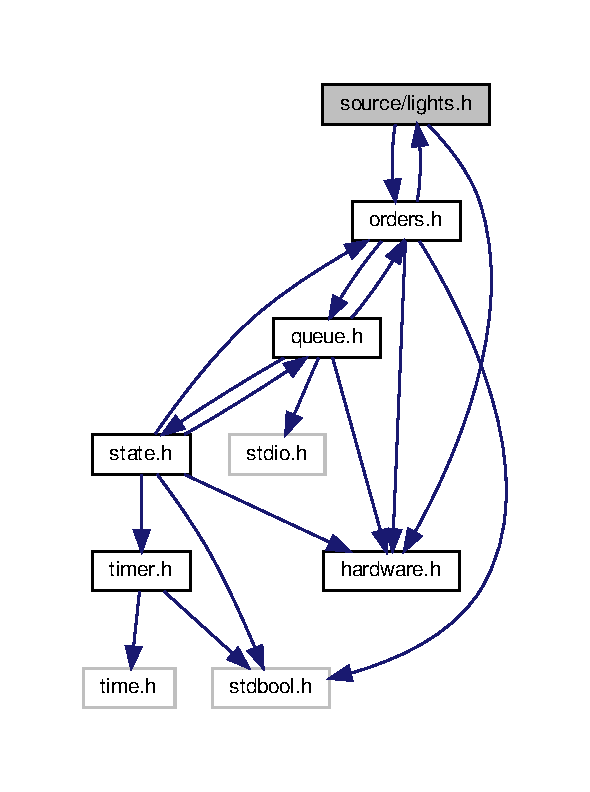
\includegraphics[width=283pt]{lights_8h__incl}
\end{center}
\end{figure}
This graph shows which files directly or indirectly include this file\+:
\nopagebreak
\begin{figure}[H]
\begin{center}
\leavevmode
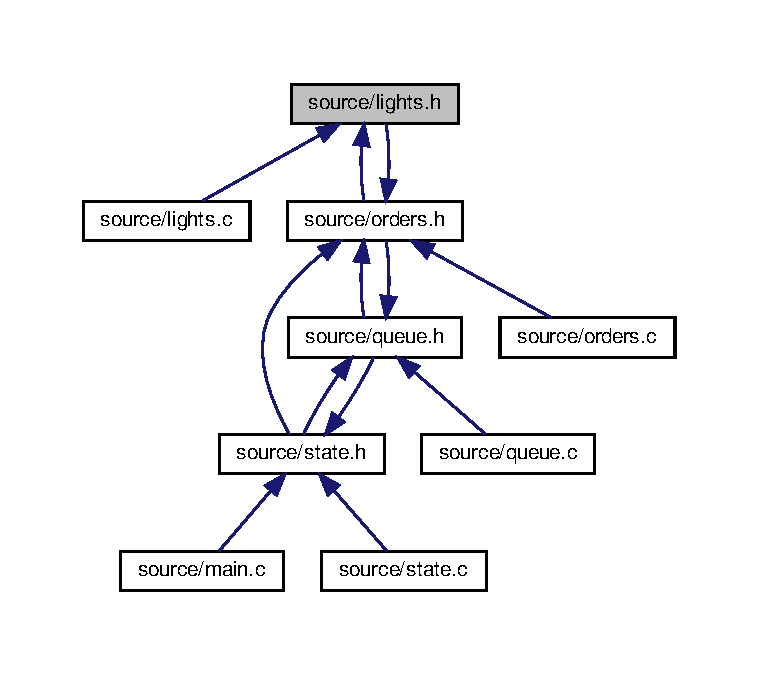
\includegraphics[width=350pt]{lights_8h__dep__incl}
\end{center}
\end{figure}
\subsection*{Functions}
\begin{DoxyCompactItemize}
\item 
\mbox{\Hypertarget{lights_8h_ac3cbb05034ff71c26f5b7eab1df24dbf}\label{lights_8h_ac3cbb05034ff71c26f5b7eab1df24dbf}} 
void \hyperlink{lights_8h_ac3cbb05034ff71c26f5b7eab1df24dbf}{set\+\_\+order\+\_\+lights} ()
\begin{DoxyCompactList}\small\item\em Iterates through all the order-\/buttons. If an order button is active, which we check by using the \hyperlink{hardware_8h_a87917f3aa093fb46ca821a400d011ee8}{hardware\+\_\+read\+\_\+order()} from \hyperlink{hardware_8h}{hardware.\+h}, the funtion will turn the light on in said button. \end{DoxyCompactList}\item 
void \hyperlink{lights_8h_a137498fd9fbbecf25ac39e9911fc07fe}{clear\+\_\+order\+\_\+lights} (int floor)
\begin{DoxyCompactList}\small\item\em Deactivate order lights on the floor specified in the parameter, by iterating through the order-\/buttons. \end{DoxyCompactList}\item 
\mbox{\Hypertarget{lights_8h_afd77151474c3e94d7c52fd75413ae3ca}\label{lights_8h_afd77151474c3e94d7c52fd75413ae3ca}} 
void \hyperlink{lights_8h_afd77151474c3e94d7c52fd75413ae3ca}{clear\+\_\+all\+\_\+order\+\_\+lights} ()
\begin{DoxyCompactList}\small\item\em By using clear\+\_\+order\+\_\+lights, this function iterates though all possible floors, deactivating the lights on all order-\/buttons. \end{DoxyCompactList}\item 
\mbox{\Hypertarget{lights_8h_ad61c6d8a7c11e4adf676c586f5391571}\label{lights_8h_ad61c6d8a7c11e4adf676c586f5391571}} 
void \hyperlink{lights_8h_ad61c6d8a7c11e4adf676c586f5391571}{on\+\_\+stop\+\_\+light} ()
\begin{DoxyCompactList}\small\item\em Activates the stop light, by calling hardware\+\_\+command\+\_\+stop\+\_\+light(1) from \hyperlink{hardware_8h}{hardware.\+h}. \end{DoxyCompactList}\item 
\mbox{\Hypertarget{lights_8h_a3b782c92ff52ddc357009fad24931271}\label{lights_8h_a3b782c92ff52ddc357009fad24931271}} 
void \hyperlink{lights_8h_a3b782c92ff52ddc357009fad24931271}{off\+\_\+stop\+\_\+light} ()
\begin{DoxyCompactList}\small\item\em Deactivates the stop light, by calling hardware\+\_\+command\+\_\+stop\+\_\+light(0) from \hyperlink{hardware_8h}{hardware.\+h}. \end{DoxyCompactList}\item 
\mbox{\Hypertarget{lights_8h_a423745a554b7b74fd8a6ee276f3ee4f6}\label{lights_8h_a423745a554b7b74fd8a6ee276f3ee4f6}} 
void \hyperlink{lights_8h_a423745a554b7b74fd8a6ee276f3ee4f6}{open\+\_\+door} ()
\begin{DoxyCompactList}\small\item\em Activates the door light, by calling hardware\+\_\+command\+\_\+door\+\_\+open(1) from \hyperlink{hardware_8h}{hardware.\+h}. \end{DoxyCompactList}\item 
\mbox{\Hypertarget{lights_8h_a7e9a332d026a32072d6080c2f1264813}\label{lights_8h_a7e9a332d026a32072d6080c2f1264813}} 
void \hyperlink{lights_8h_a7e9a332d026a32072d6080c2f1264813}{close\+\_\+door} ()
\begin{DoxyCompactList}\small\item\em Deactivates the door light, by calling hardware\+\_\+command\+\_\+door\+\_\+open(0) from \hyperlink{hardware_8h}{hardware.\+h}. \end{DoxyCompactList}\end{DoxyCompactItemize}


\subsection{Detailed Description}
A library for doing operations on the lights on the floor-\/panel. 



\subsection{Function Documentation}
\mbox{\Hypertarget{lights_8h_a137498fd9fbbecf25ac39e9911fc07fe}\label{lights_8h_a137498fd9fbbecf25ac39e9911fc07fe}} 
\index{lights.\+h@{lights.\+h}!clear\+\_\+order\+\_\+lights@{clear\+\_\+order\+\_\+lights}}
\index{clear\+\_\+order\+\_\+lights@{clear\+\_\+order\+\_\+lights}!lights.\+h@{lights.\+h}}
\subsubsection{\texorpdfstring{clear\+\_\+order\+\_\+lights()}{clear\_order\_lights()}}
{\footnotesize\ttfamily void clear\+\_\+order\+\_\+lights (\begin{DoxyParamCaption}\item[{int}]{floor }\end{DoxyParamCaption})}



Deactivate order lights on the floor specified in the parameter, by iterating through the order-\/buttons. 


\begin{DoxyParams}[1]{Parameters}
\mbox{\tt in}  & {\em floor} & The given floor that will have it\textquotesingle{}s order-\/buttons lights deactivated. \\
\hline
\end{DoxyParams}


Definition at line 15 of file lights.\+c.


\hypertarget{orders_8h}{}\section{source/orders.h File Reference}
\label{orders_8h}\index{source/orders.\+h@{source/orders.\+h}}


Implementation of management of orders.  


{\ttfamily \#include \char`\"{}stdbool.\+h\char`\"{}}\newline
{\ttfamily \#include \char`\"{}hardware.\+h\char`\"{}}\newline
{\ttfamily \#include \char`\"{}queue.\+h\char`\"{}}\newline
{\ttfamily \#include \char`\"{}lights.\+h\char`\"{}}\newline
Include dependency graph for orders.\+h\+:
\nopagebreak
\begin{figure}[H]
\begin{center}
\leavevmode
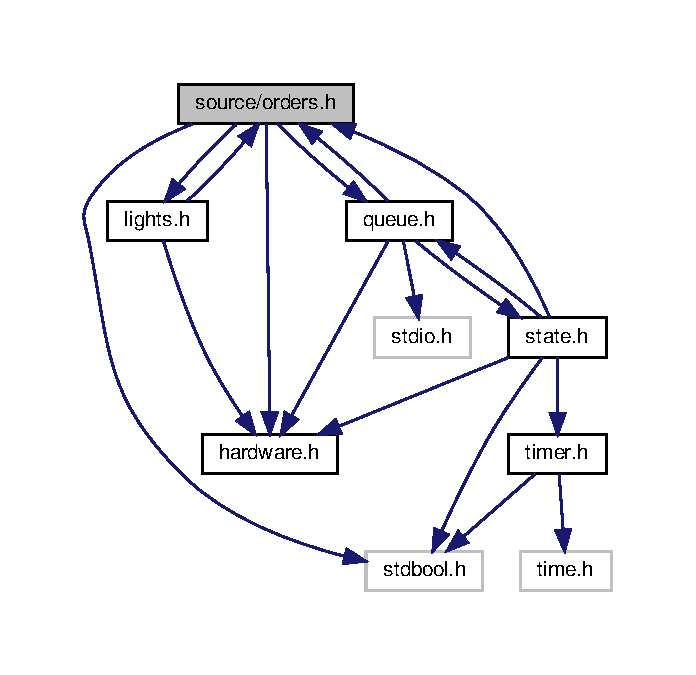
\includegraphics[width=334pt]{orders_8h__incl}
\end{center}
\end{figure}
This graph shows which files directly or indirectly include this file\+:
\nopagebreak
\begin{figure}[H]
\begin{center}
\leavevmode
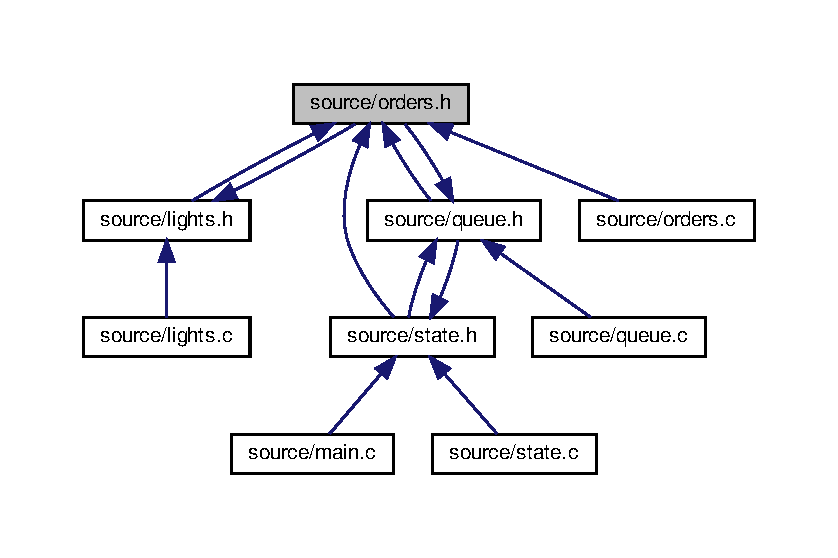
\includegraphics[width=350pt]{orders_8h__dep__incl}
\end{center}
\end{figure}
\subsection*{Functions}
\begin{DoxyCompactItemize}
\item 
\mbox{\Hypertarget{orders_8h_abc9f9064a2a12b6206c222bb3191b38e}\label{orders_8h_abc9f9064a2a12b6206c222bb3191b38e}} 
\hyperlink{hardware_8h_a796a8de8ce0ae769d7dbd3327a7bdbe7}{Hardware\+Order} {\bfseries get\+\_\+hardwareorder} (int button)
\item 
\mbox{\Hypertarget{orders_8h_a061efad066833f37bb777acc0322e140}\label{orders_8h_a061efad066833f37bb777acc0322e140}} 
void \hyperlink{orders_8h_a061efad066833f37bb777acc0322e140}{initialize\+\_\+order\+\_\+list} ()
\begin{DoxyCompactList}\small\item\em Initializes the order-\/array, makes an empty array\+: orders\mbox{[}floor\mbox{]}\mbox{[}button\mbox{]}. \end{DoxyCompactList}\item 
\mbox{\Hypertarget{orders_8h_a04fb5ec6aa91c0a9aca9a62bd8f77dc7}\label{orders_8h_a04fb5ec6aa91c0a9aca9a62bd8f77dc7}} 
void \hyperlink{orders_8h_a04fb5ec6aa91c0a9aca9a62bd8f77dc7}{set\+\_\+orders} ()
\begin{DoxyCompactList}\small\item\em Iterates through all the buttons on the floor-\/panel. If a button is pushed, the corresponding place in the array will be set to active. \end{DoxyCompactList}\item 
int \hyperlink{orders_8h_a197b5cc8b46cfde2a097c852b01d1c4b}{get\+\_\+order} (int floor, int button)
\begin{DoxyCompactList}\small\item\em Returns the given value saved in the specified place in the orders-\/array. \end{DoxyCompactList}\item 
void \hyperlink{orders_8h_a34eb2168d05d8b42d28ce98905a5976e}{clear\+\_\+orders\+\_\+on\+\_\+floor} (int floor)
\begin{DoxyCompactList}\small\item\em Clears all order on a given floor. \end{DoxyCompactList}\item 
\mbox{\Hypertarget{orders_8h_a6206e5203639ca23d84820e2ffb108a3}\label{orders_8h_a6206e5203639ca23d84820e2ffb108a3}} 
void \hyperlink{orders_8h_a6206e5203639ca23d84820e2ffb108a3}{clear\+\_\+all\+\_\+orders} ()
\begin{DoxyCompactList}\small\item\em Clears all orders by iterating \hyperlink{orders_8h_a34eb2168d05d8b42d28ce98905a5976e}{clear\+\_\+orders\+\_\+on\+\_\+floor(int floor)} through all floors. \end{DoxyCompactList}\item 
int \hyperlink{orders_8h_a37c377d96551aaf01823c12ff475f215}{check\+\_\+order\+\_\+floor} (int floor)
\begin{DoxyCompactList}\small\item\em If floor != (-\/1), if the elevator is not in an undefined position, check if the there is an active order on the current floor. \end{DoxyCompactList}\item 
int \hyperlink{orders_8h_afa04aae38011cd957102bb9da18d9907}{check\+\_\+all\+\_\+order} ()
\begin{DoxyCompactList}\small\item\em Check for all active orders by iterating through all existing floors. For each iteration, checks if \hyperlink{orders_8h_a37c377d96551aaf01823c12ff475f215}{check\+\_\+order\+\_\+floor(int floor)} == 1. If true, return 1. False, return 0. \end{DoxyCompactList}\item 
int \hyperlink{orders_8h_ab4742330b65b88c1dd2e9942e295c3a1}{check\+\_\+order\+\_\+above} ()
\begin{DoxyCompactList}\small\item\em Check for all active orders above current floor by iterating between current floor and top floor. For each iteration, checks if \hyperlink{orders_8h_a37c377d96551aaf01823c12ff475f215}{check\+\_\+order\+\_\+floor(int floor)} == 1. If true, return 1. False, return 0. \end{DoxyCompactList}\item 
int \hyperlink{orders_8h_a611521170cfe0b7438d01e2ab8269fee}{check\+\_\+order\+\_\+below} ()
\begin{DoxyCompactList}\small\item\em Check for all active orders below current floor by iterating between ground floor and current floor. For each iteration, checks if \hyperlink{orders_8h_a37c377d96551aaf01823c12ff475f215}{check\+\_\+order\+\_\+floor(int floor)} == 1. If true, return 1. False, return 0. \end{DoxyCompactList}\item 
int \hyperlink{orders_8h_acf6b7bcd3a2deb033e834cbc58fba3b1}{check\+\_\+order\+\_\+below\+\_\+current\+\_\+floor} ()
\begin{DoxyCompactList}\small\item\em Check for all active orders below current floor by iterating between ground floor and the floor directly under the current floor. Used in \hyperlink{queue_8h_a8738e0662c2d336c7573829c9be0e44c}{check\+\_\+priority\+\_\+down()} in \hyperlink{queue_8c_source}{queue.\+c}. For each iteration, checks if \hyperlink{orders_8h_a37c377d96551aaf01823c12ff475f215}{check\+\_\+order\+\_\+floor(int floor)} == 1. If true, return 1. False, return 0. \end{DoxyCompactList}\item 
int \hyperlink{orders_8h_aa3961df9a9b23e57a65171091b3885f6}{find\+\_\+floor\+\_\+with\+\_\+order} ()
\begin{DoxyCompactList}\small\item\em Finds a floor with an active order. Uses \hyperlink{orders_8h_a37c377d96551aaf01823c12ff475f215}{check\+\_\+order\+\_\+floor(int floor)} by iterating through all floors, and returning the floor with an active order. \end{DoxyCompactList}\end{DoxyCompactItemize}


\subsection{Detailed Description}
Implementation of management of orders. 



\subsection{Function Documentation}
\mbox{\Hypertarget{orders_8h_afa04aae38011cd957102bb9da18d9907}\label{orders_8h_afa04aae38011cd957102bb9da18d9907}} 
\index{orders.\+h@{orders.\+h}!check\+\_\+all\+\_\+order@{check\+\_\+all\+\_\+order}}
\index{check\+\_\+all\+\_\+order@{check\+\_\+all\+\_\+order}!orders.\+h@{orders.\+h}}
\subsubsection{\texorpdfstring{check\+\_\+all\+\_\+order()}{check\_all\_order()}}
{\footnotesize\ttfamily int check\+\_\+all\+\_\+order (\begin{DoxyParamCaption}{ }\end{DoxyParamCaption})}



Check for all active orders by iterating through all existing floors. For each iteration, checks if \hyperlink{orders_8h_a37c377d96551aaf01823c12ff475f215}{check\+\_\+order\+\_\+floor(int floor)} == 1. If true, return 1. False, return 0. 

\begin{DoxyReturn}{Returns}
1, if there is an active order on any of the floors. 0, if there are no active orders. 
\end{DoxyReturn}


Definition at line 79 of file orders.\+c.

\mbox{\Hypertarget{orders_8h_ab4742330b65b88c1dd2e9942e295c3a1}\label{orders_8h_ab4742330b65b88c1dd2e9942e295c3a1}} 
\index{orders.\+h@{orders.\+h}!check\+\_\+order\+\_\+above@{check\+\_\+order\+\_\+above}}
\index{check\+\_\+order\+\_\+above@{check\+\_\+order\+\_\+above}!orders.\+h@{orders.\+h}}
\subsubsection{\texorpdfstring{check\+\_\+order\+\_\+above()}{check\_order\_above()}}
{\footnotesize\ttfamily int check\+\_\+order\+\_\+above (\begin{DoxyParamCaption}{ }\end{DoxyParamCaption})}



Check for all active orders above current floor by iterating between current floor and top floor. For each iteration, checks if \hyperlink{orders_8h_a37c377d96551aaf01823c12ff475f215}{check\+\_\+order\+\_\+floor(int floor)} == 1. If true, return 1. False, return 0. 

\begin{DoxyReturn}{Returns}
1, if there is an active order on any of the floors above. 0, otherwise. 
\end{DoxyReturn}


Definition at line 90 of file orders.\+c.

\mbox{\Hypertarget{orders_8h_a611521170cfe0b7438d01e2ab8269fee}\label{orders_8h_a611521170cfe0b7438d01e2ab8269fee}} 
\index{orders.\+h@{orders.\+h}!check\+\_\+order\+\_\+below@{check\+\_\+order\+\_\+below}}
\index{check\+\_\+order\+\_\+below@{check\+\_\+order\+\_\+below}!orders.\+h@{orders.\+h}}
\subsubsection{\texorpdfstring{check\+\_\+order\+\_\+below()}{check\_order\_below()}}
{\footnotesize\ttfamily int check\+\_\+order\+\_\+below (\begin{DoxyParamCaption}{ }\end{DoxyParamCaption})}



Check for all active orders below current floor by iterating between ground floor and current floor. For each iteration, checks if \hyperlink{orders_8h_a37c377d96551aaf01823c12ff475f215}{check\+\_\+order\+\_\+floor(int floor)} == 1. If true, return 1. False, return 0. 

\begin{DoxyReturn}{Returns}
1, if there is an active order on any of the floors below. 0, otherwise. 
\end{DoxyReturn}


Definition at line 100 of file orders.\+c.

\mbox{\Hypertarget{orders_8h_acf6b7bcd3a2deb033e834cbc58fba3b1}\label{orders_8h_acf6b7bcd3a2deb033e834cbc58fba3b1}} 
\index{orders.\+h@{orders.\+h}!check\+\_\+order\+\_\+below\+\_\+current\+\_\+floor@{check\+\_\+order\+\_\+below\+\_\+current\+\_\+floor}}
\index{check\+\_\+order\+\_\+below\+\_\+current\+\_\+floor@{check\+\_\+order\+\_\+below\+\_\+current\+\_\+floor}!orders.\+h@{orders.\+h}}
\subsubsection{\texorpdfstring{check\+\_\+order\+\_\+below\+\_\+current\+\_\+floor()}{check\_order\_below\_current\_floor()}}
{\footnotesize\ttfamily int check\+\_\+order\+\_\+below\+\_\+current\+\_\+floor (\begin{DoxyParamCaption}{ }\end{DoxyParamCaption})}



Check for all active orders below current floor by iterating between ground floor and the floor directly under the current floor. Used in \hyperlink{queue_8h_a8738e0662c2d336c7573829c9be0e44c}{check\+\_\+priority\+\_\+down()} in \hyperlink{queue_8c_source}{queue.\+c}. For each iteration, checks if \hyperlink{orders_8h_a37c377d96551aaf01823c12ff475f215}{check\+\_\+order\+\_\+floor(int floor)} == 1. If true, return 1. False, return 0. 

\begin{DoxyReturn}{Returns}
1, if there is an active order on any of the floors below. 0, otherwise. 
\end{DoxyReturn}


Definition at line 110 of file orders.\+c.

\mbox{\Hypertarget{orders_8h_a37c377d96551aaf01823c12ff475f215}\label{orders_8h_a37c377d96551aaf01823c12ff475f215}} 
\index{orders.\+h@{orders.\+h}!check\+\_\+order\+\_\+floor@{check\+\_\+order\+\_\+floor}}
\index{check\+\_\+order\+\_\+floor@{check\+\_\+order\+\_\+floor}!orders.\+h@{orders.\+h}}
\subsubsection{\texorpdfstring{check\+\_\+order\+\_\+floor()}{check\_order\_floor()}}
{\footnotesize\ttfamily int check\+\_\+order\+\_\+floor (\begin{DoxyParamCaption}\item[{int}]{floor }\end{DoxyParamCaption})}



If floor != (-\/1), if the elevator is not in an undefined position, check if the there is an active order on the current floor. 


\begin{DoxyParams}[1]{Parameters}
\mbox{\tt in}  & {\em floor} & The current floor.\\
\hline
\end{DoxyParams}
\begin{DoxyReturn}{Returns}
0, if floor != (-\/1), or if there aren\textquotesingle{}t active orders on floor. 1, there is an active order on the current floor. 
\end{DoxyReturn}


Definition at line 64 of file orders.\+c.

\mbox{\Hypertarget{orders_8h_a34eb2168d05d8b42d28ce98905a5976e}\label{orders_8h_a34eb2168d05d8b42d28ce98905a5976e}} 
\index{orders.\+h@{orders.\+h}!clear\+\_\+orders\+\_\+on\+\_\+floor@{clear\+\_\+orders\+\_\+on\+\_\+floor}}
\index{clear\+\_\+orders\+\_\+on\+\_\+floor@{clear\+\_\+orders\+\_\+on\+\_\+floor}!orders.\+h@{orders.\+h}}
\subsubsection{\texorpdfstring{clear\+\_\+orders\+\_\+on\+\_\+floor()}{clear\_orders\_on\_floor()}}
{\footnotesize\ttfamily void clear\+\_\+orders\+\_\+on\+\_\+floor (\begin{DoxyParamCaption}\item[{int}]{floor }\end{DoxyParamCaption})}



Clears all order on a given floor. 


\begin{DoxyParams}[1]{Parameters}
\mbox{\tt in}  & {\em floor} & The specified floor. \\
\hline
\end{DoxyParams}


Definition at line 49 of file orders.\+c.

\mbox{\Hypertarget{orders_8h_aa3961df9a9b23e57a65171091b3885f6}\label{orders_8h_aa3961df9a9b23e57a65171091b3885f6}} 
\index{orders.\+h@{orders.\+h}!find\+\_\+floor\+\_\+with\+\_\+order@{find\+\_\+floor\+\_\+with\+\_\+order}}
\index{find\+\_\+floor\+\_\+with\+\_\+order@{find\+\_\+floor\+\_\+with\+\_\+order}!orders.\+h@{orders.\+h}}
\subsubsection{\texorpdfstring{find\+\_\+floor\+\_\+with\+\_\+order()}{find\_floor\_with\_order()}}
{\footnotesize\ttfamily int find\+\_\+floor\+\_\+with\+\_\+order (\begin{DoxyParamCaption}{ }\end{DoxyParamCaption})}



Finds a floor with an active order. Uses \hyperlink{orders_8h_a37c377d96551aaf01823c12ff475f215}{check\+\_\+order\+\_\+floor(int floor)} by iterating through all floors, and returning the floor with an active order. 

\begin{DoxyReturn}{Returns}
the floor with an active order, 1 if invalid floor. 
\end{DoxyReturn}


Definition at line 122 of file orders.\+c.

\mbox{\Hypertarget{orders_8h_a197b5cc8b46cfde2a097c852b01d1c4b}\label{orders_8h_a197b5cc8b46cfde2a097c852b01d1c4b}} 
\index{orders.\+h@{orders.\+h}!get\+\_\+order@{get\+\_\+order}}
\index{get\+\_\+order@{get\+\_\+order}!orders.\+h@{orders.\+h}}
\subsubsection{\texorpdfstring{get\+\_\+order()}{get\_order()}}
{\footnotesize\ttfamily int get\+\_\+order (\begin{DoxyParamCaption}\item[{int}]{floor,  }\item[{int}]{button }\end{DoxyParamCaption})}



Returns the given value saved in the specified place in the orders-\/array. 


\begin{DoxyParams}[1]{Parameters}
\mbox{\tt in}  & {\em floor} & The specified floor \\
\hline
\mbox{\tt in}  & {\em button} & The specified order-\/button\\
\hline
\end{DoxyParams}
\begin{DoxyReturn}{Returns}
orders\mbox{[}floor\mbox{]}\mbox{[}button\mbox{]}, which is 1 if it has an active order, 0 otherwise 
\end{DoxyReturn}


Definition at line 44 of file orders.\+c.


\hypertarget{queue_8h}{}\section{source/queue.h File Reference}
\label{queue_8h}\index{source/queue.\+h@{source/queue.\+h}}


Library for the implementation of queue.  


{\ttfamily \#include \char`\"{}hardware.\+h\char`\"{}}\newline
{\ttfamily \#include \char`\"{}orders.\+h\char`\"{}}\newline
{\ttfamily \#include \char`\"{}stdio.\+h\char`\"{}}\newline
{\ttfamily \#include \char`\"{}state.\+h\char`\"{}}\newline
Include dependency graph for queue.\+h\+:
\nopagebreak
\begin{figure}[H]
\begin{center}
\leavevmode
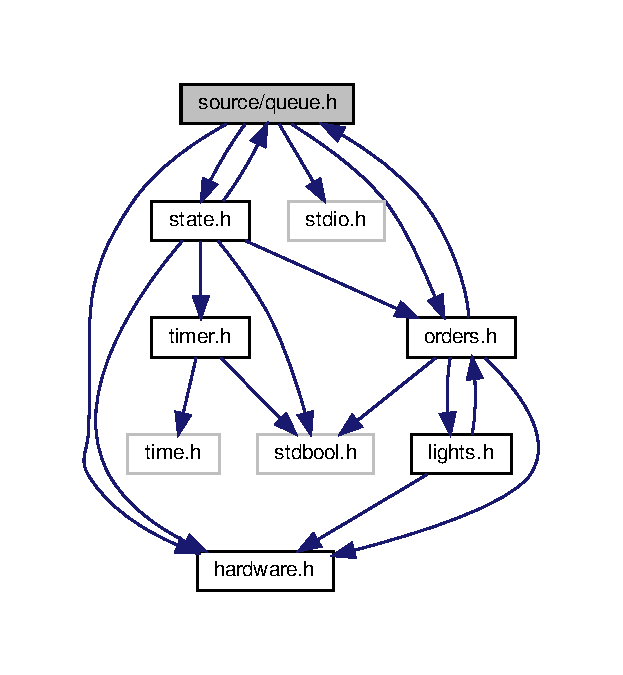
\includegraphics[width=299pt]{queue_8h__incl}
\end{center}
\end{figure}
This graph shows which files directly or indirectly include this file\+:
\nopagebreak
\begin{figure}[H]
\begin{center}
\leavevmode
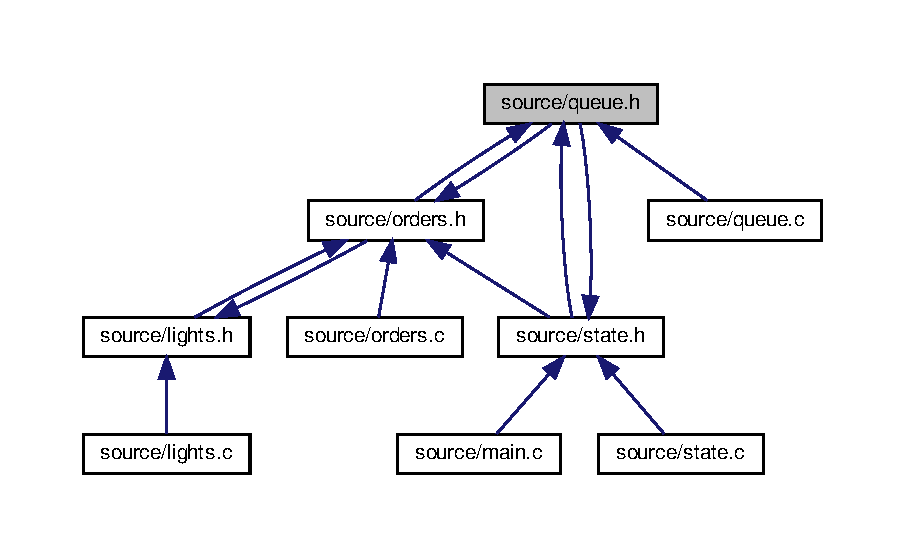
\includegraphics[width=350pt]{queue_8h__dep__incl}
\end{center}
\end{figure}
\subsection*{Functions}
\begin{DoxyCompactItemize}
\item 
int \hyperlink{queue_8h_ab6d5385762b69dab12732efd71fb09cd}{current\+\_\+position} ()
\begin{DoxyCompactList}\small\item\em Finds the current position. \end{DoxyCompactList}\item 
\mbox{\Hypertarget{queue_8h_a178e558cfd6872984c2d29792a508e9b}\label{queue_8h_a178e558cfd6872984c2d29792a508e9b}} 
void \hyperlink{queue_8h_a178e558cfd6872984c2d29792a508e9b}{set\+\_\+last\+\_\+position} ()
\begin{DoxyCompactList}\small\item\em The last\+\_\+position variable is updated When the elevator moves to a defined floor, last\+\_\+position = \hyperlink{queue_8h_ab6d5385762b69dab12732efd71fb09cd}{current\+\_\+position()} \end{DoxyCompactList}\item 
int \hyperlink{queue_8h_a27076904adf2475044d85701f2facc27}{get\+\_\+last\+\_\+position} ()
\begin{DoxyCompactList}\small\item\em Returns last\+\_\+position. \end{DoxyCompactList}\item 
void \hyperlink{queue_8h_acf6f3f01ccc5d2cc5678499e4a992400}{set\+\_\+current\+\_\+direction} (int direction)
\begin{DoxyCompactList}\small\item\em Changes current\+\_\+direction to direction. \end{DoxyCompactList}\item 
void \hyperlink{queue_8h_af7aa9046b156b74a3b2aebd620fc3e72}{set\+\_\+start\+\_\+direction} (int new\+\_\+floor)
\begin{DoxyCompactList}\small\item\em Chooses the starting direction, when order is placed in idle. \end{DoxyCompactList}\item 
int \hyperlink{queue_8h_ac426009b9dd5bd9bc76949a454a320a6}{get\+\_\+current\+\_\+direction} ()
\begin{DoxyCompactList}\small\item\em Returns current\+\_\+direction. \end{DoxyCompactList}\item 
int \hyperlink{queue_8h_ac299892189fe5e25366c96583ce71110}{find\+\_\+direction\+\_\+when\+\_\+stop} ()
\begin{DoxyCompactList}\small\item\em Decides te new direction, when order is placed in state Stop\+Shaft. Uses new\+\_\+floor and last\+\_\+position to decide which floors the elevator is located between. Chooses the direction based on this. \end{DoxyCompactList}\item 
int \hyperlink{queue_8h_aa7ed6c09f3841bf8eff8018173a95c1a}{check\+\_\+priority\+\_\+up} ()
\begin{DoxyCompactList}\small\item\em Decide if Down-\/orders should be ignored when movement is Up. \end{DoxyCompactList}\item 
void \hyperlink{queue_8h_ab08043d789b16601723fdac11bdf827c}{movement\+\_\+up} ()
\begin{DoxyCompactList}\small\item\em Decides if the elevator should stop, continue up or change direction. Moves up until elevator reaches floor with order. Stops, clear orders on floor and lights. Set timer. Checks if there are more orders above. If yes, continues up. If not, checks if there are more orders below. If yes, changes direction down. Otherwise, changes state to Idle. \end{DoxyCompactList}\item 
int \hyperlink{queue_8h_a8738e0662c2d336c7573829c9be0e44c}{check\+\_\+priority\+\_\+down} ()
\begin{DoxyCompactList}\small\item\em Decide if Up-\/orders should be ignored when movement is Down. \end{DoxyCompactList}\item 
\mbox{\Hypertarget{queue_8h_acb3c47304ad272e106be094200689350}\label{queue_8h_acb3c47304ad272e106be094200689350}} 
void \hyperlink{queue_8h_acb3c47304ad272e106be094200689350}{movement\+\_\+down} ()
\begin{DoxyCompactList}\small\item\em Decides if the elevator should stop, continue up or change direction. Moves down until elevator reaches floor with order. Stops, clear orders on floor and lights. Set timer. Checks if there are more orders below. If yes, continues down. If not, checks if there are more orders above. If yes, changes direction up. Otherwise, changes state to Idle. \end{DoxyCompactList}\item 
\mbox{\Hypertarget{queue_8h_a05f4d4ebc3e0b18fc70f3902771cce28}\label{queue_8h_a05f4d4ebc3e0b18fc70f3902771cce28}} 
void \hyperlink{queue_8h_a05f4d4ebc3e0b18fc70f3902771cce28}{queue\+\_\+manager} ()
\begin{DoxyCompactList}\small\item\em Decides queue based on current\+\_\+direction. If the direction is up, calls \hyperlink{queue_8h_ab08043d789b16601723fdac11bdf827c}{movement\+\_\+up()}, if direction is down, calls \hyperlink{queue_8h_acb3c47304ad272e106be094200689350}{movement\+\_\+down()}. If the order is on current floor, stays on current floor, change state to Wait after set\+\_\+timer(). \end{DoxyCompactList}\end{DoxyCompactItemize}


\subsection{Detailed Description}
Library for the implementation of queue. 



\subsection{Function Documentation}
\mbox{\Hypertarget{queue_8h_a8738e0662c2d336c7573829c9be0e44c}\label{queue_8h_a8738e0662c2d336c7573829c9be0e44c}} 
\index{queue.\+h@{queue.\+h}!check\+\_\+priority\+\_\+down@{check\+\_\+priority\+\_\+down}}
\index{check\+\_\+priority\+\_\+down@{check\+\_\+priority\+\_\+down}!queue.\+h@{queue.\+h}}
\subsubsection{\texorpdfstring{check\+\_\+priority\+\_\+down()}{check\_priority\_down()}}
{\footnotesize\ttfamily int check\+\_\+priority\+\_\+down (\begin{DoxyParamCaption}{ }\end{DoxyParamCaption})}



Decide if Up-\/orders should be ignored when movement is Down. 

\begin{DoxyReturn}{Returns}
1 if it should be ignored, 0 otherwise 
\end{DoxyReturn}


Definition at line 105 of file queue.\+c.

\mbox{\Hypertarget{queue_8h_aa7ed6c09f3841bf8eff8018173a95c1a}\label{queue_8h_aa7ed6c09f3841bf8eff8018173a95c1a}} 
\index{queue.\+h@{queue.\+h}!check\+\_\+priority\+\_\+up@{check\+\_\+priority\+\_\+up}}
\index{check\+\_\+priority\+\_\+up@{check\+\_\+priority\+\_\+up}!queue.\+h@{queue.\+h}}
\subsubsection{\texorpdfstring{check\+\_\+priority\+\_\+up()}{check\_priority\_up()}}
{\footnotesize\ttfamily int check\+\_\+priority\+\_\+up (\begin{DoxyParamCaption}{ }\end{DoxyParamCaption})}



Decide if Down-\/orders should be ignored when movement is Up. 

\begin{DoxyReturn}{Returns}
1 if it should be ignored, 0 otherwise 
\end{DoxyReturn}


Definition at line 72 of file queue.\+c.

\mbox{\Hypertarget{queue_8h_ab6d5385762b69dab12732efd71fb09cd}\label{queue_8h_ab6d5385762b69dab12732efd71fb09cd}} 
\index{queue.\+h@{queue.\+h}!current\+\_\+position@{current\+\_\+position}}
\index{current\+\_\+position@{current\+\_\+position}!queue.\+h@{queue.\+h}}
\subsubsection{\texorpdfstring{current\+\_\+position()}{current\_position()}}
{\footnotesize\ttfamily int current\+\_\+position (\begin{DoxyParamCaption}{ }\end{DoxyParamCaption})}



Finds the current position. 

\begin{DoxyReturn}{Returns}
-\/1, if in an undefined floor, the floor number if in a defined floor. 
\end{DoxyReturn}


Definition at line 6 of file queue.\+c.

\mbox{\Hypertarget{queue_8h_ac299892189fe5e25366c96583ce71110}\label{queue_8h_ac299892189fe5e25366c96583ce71110}} 
\index{queue.\+h@{queue.\+h}!find\+\_\+direction\+\_\+when\+\_\+stop@{find\+\_\+direction\+\_\+when\+\_\+stop}}
\index{find\+\_\+direction\+\_\+when\+\_\+stop@{find\+\_\+direction\+\_\+when\+\_\+stop}!queue.\+h@{queue.\+h}}
\subsubsection{\texorpdfstring{find\+\_\+direction\+\_\+when\+\_\+stop()}{find\_direction\_when\_stop()}}
{\footnotesize\ttfamily int find\+\_\+direction\+\_\+when\+\_\+stop (\begin{DoxyParamCaption}{ }\end{DoxyParamCaption})}



Decides te new direction, when order is placed in state Stop\+Shaft. Uses new\+\_\+floor and last\+\_\+position to decide which floors the elevator is located between. Chooses the direction based on this. 

\begin{DoxyReturn}{Returns}
-\/1 = direction down, 1 = direction up. 

1 if unexpected event. 
\end{DoxyReturn}


Definition at line 52 of file queue.\+c.

\mbox{\Hypertarget{queue_8h_ac426009b9dd5bd9bc76949a454a320a6}\label{queue_8h_ac426009b9dd5bd9bc76949a454a320a6}} 
\index{queue.\+h@{queue.\+h}!get\+\_\+current\+\_\+direction@{get\+\_\+current\+\_\+direction}}
\index{get\+\_\+current\+\_\+direction@{get\+\_\+current\+\_\+direction}!queue.\+h@{queue.\+h}}
\subsubsection{\texorpdfstring{get\+\_\+current\+\_\+direction()}{get\_current\_direction()}}
{\footnotesize\ttfamily int get\+\_\+current\+\_\+direction (\begin{DoxyParamCaption}{ }\end{DoxyParamCaption})}



Returns current\+\_\+direction. 

\begin{DoxyReturn}{Returns}
current\+\_\+direction 
\end{DoxyReturn}


Definition at line 47 of file queue.\+c.

\mbox{\Hypertarget{queue_8h_a27076904adf2475044d85701f2facc27}\label{queue_8h_a27076904adf2475044d85701f2facc27}} 
\index{queue.\+h@{queue.\+h}!get\+\_\+last\+\_\+position@{get\+\_\+last\+\_\+position}}
\index{get\+\_\+last\+\_\+position@{get\+\_\+last\+\_\+position}!queue.\+h@{queue.\+h}}
\subsubsection{\texorpdfstring{get\+\_\+last\+\_\+position()}{get\_last\_position()}}
{\footnotesize\ttfamily int get\+\_\+last\+\_\+position (\begin{DoxyParamCaption}{ }\end{DoxyParamCaption})}



Returns last\+\_\+position. 

\begin{DoxyReturn}{Returns}
last\+\_\+position 
\end{DoxyReturn}


Definition at line 24 of file queue.\+c.

\mbox{\Hypertarget{queue_8h_ab08043d789b16601723fdac11bdf827c}\label{queue_8h_ab08043d789b16601723fdac11bdf827c}} 
\index{queue.\+h@{queue.\+h}!movement\+\_\+up@{movement\+\_\+up}}
\index{movement\+\_\+up@{movement\+\_\+up}!queue.\+h@{queue.\+h}}
\subsubsection{\texorpdfstring{movement\+\_\+up()}{movement\_up()}}
{\footnotesize\ttfamily void movement\+\_\+up (\begin{DoxyParamCaption}{ }\end{DoxyParamCaption})}



Decides if the elevator should stop, continue up or change direction. Moves up until elevator reaches floor with order. Stops, clear orders on floor and lights. Set timer. Checks if there are more orders above. If yes, continues up. If not, checks if there are more orders below. If yes, changes direction down. Otherwise, changes state to Idle. 



Definition at line 77 of file queue.\+c.

\mbox{\Hypertarget{queue_8h_acf6f3f01ccc5d2cc5678499e4a992400}\label{queue_8h_acf6f3f01ccc5d2cc5678499e4a992400}} 
\index{queue.\+h@{queue.\+h}!set\+\_\+current\+\_\+direction@{set\+\_\+current\+\_\+direction}}
\index{set\+\_\+current\+\_\+direction@{set\+\_\+current\+\_\+direction}!queue.\+h@{queue.\+h}}
\subsubsection{\texorpdfstring{set\+\_\+current\+\_\+direction()}{set\_current\_direction()}}
{\footnotesize\ttfamily void set\+\_\+current\+\_\+direction (\begin{DoxyParamCaption}\item[{int}]{direction }\end{DoxyParamCaption})}



Changes current\+\_\+direction to direction. 


\begin{DoxyParams}[1]{Parameters}
\mbox{\tt in}  & {\em direction} & \\
\hline
\end{DoxyParams}


Definition at line 29 of file queue.\+c.

\mbox{\Hypertarget{queue_8h_af7aa9046b156b74a3b2aebd620fc3e72}\label{queue_8h_af7aa9046b156b74a3b2aebd620fc3e72}} 
\index{queue.\+h@{queue.\+h}!set\+\_\+start\+\_\+direction@{set\+\_\+start\+\_\+direction}}
\index{set\+\_\+start\+\_\+direction@{set\+\_\+start\+\_\+direction}!queue.\+h@{queue.\+h}}
\subsubsection{\texorpdfstring{set\+\_\+start\+\_\+direction()}{set\_start\_direction()}}
{\footnotesize\ttfamily void set\+\_\+start\+\_\+direction (\begin{DoxyParamCaption}\item[{int}]{new\+\_\+floor }\end{DoxyParamCaption})}



Chooses the starting direction, when order is placed in idle. 


\begin{DoxyParams}[1]{Parameters}
\mbox{\tt in}  & {\em new\+\_\+floor} & The ordered floor \\
\hline
\end{DoxyParams}


Definition at line 34 of file queue.\+c.


\hypertarget{state_8h}{}\section{source/state.h File Reference}
\label{state_8h}\index{source/state.\+h@{source/state.\+h}}


Library for the implementation of the State Machine.  


{\ttfamily \#include \char`\"{}hardware.\+h\char`\"{}}\newline
{\ttfamily \#include \char`\"{}timer.\+h\char`\"{}}\newline
{\ttfamily \#include \char`\"{}orders.\+h\char`\"{}}\newline
{\ttfamily \#include \char`\"{}queue.\+h\char`\"{}}\newline
{\ttfamily \#include $<$stdbool.\+h$>$}\newline
Include dependency graph for state.\+h\+:
\nopagebreak
\begin{figure}[H]
\begin{center}
\leavevmode
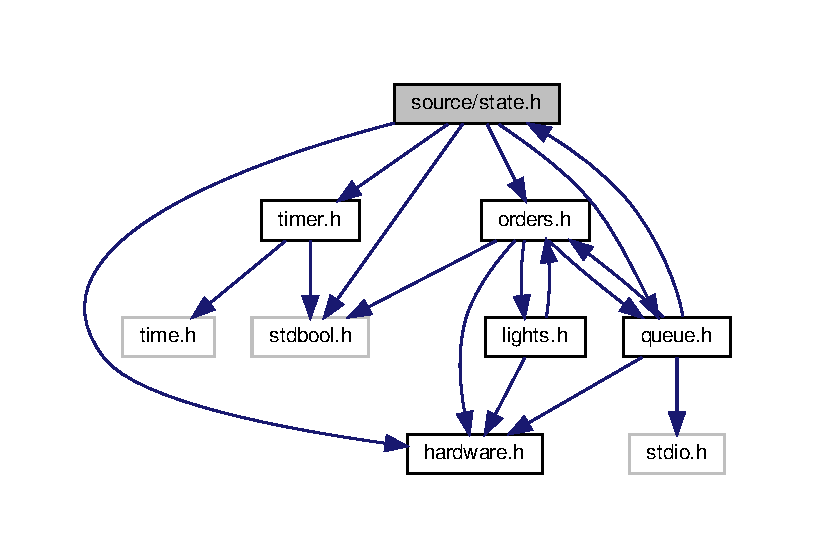
\includegraphics[width=350pt]{state_8h__incl}
\end{center}
\end{figure}
This graph shows which files directly or indirectly include this file\+:
\nopagebreak
\begin{figure}[H]
\begin{center}
\leavevmode
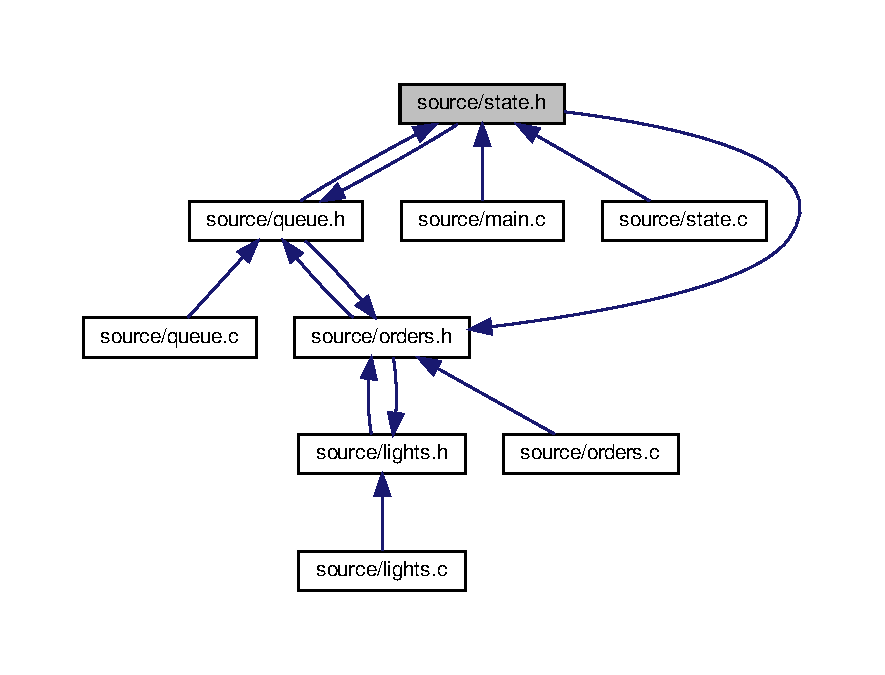
\includegraphics[width=350pt]{state_8h__dep__incl}
\end{center}
\end{figure}
\subsection*{Typedefs}
\begin{DoxyCompactItemize}
\item 
\mbox{\Hypertarget{state_8h_ae3081d55e54214abe932e6c511d6cac2}\label{state_8h_ae3081d55e54214abe932e6c511d6cac2}} 
typedef enum State {\bfseries state}
\end{DoxyCompactItemize}
\subsection*{Enumerations}
\begin{DoxyCompactItemize}
\item 
\mbox{\Hypertarget{state_8h_a5d74787dedbc4e11c1ab15bf487e61f8}\label{state_8h_a5d74787dedbc4e11c1ab15bf487e61f8}} 
enum {\bfseries State} \{ \newline
{\bfseries Idle}, 
{\bfseries Move}, 
{\bfseries Wait}, 
{\bfseries Stop\+Floor}, 
\newline
{\bfseries Stop\+Shaft}
 \}
\end{DoxyCompactItemize}
\subsection*{Functions}
\begin{DoxyCompactItemize}
\item 
\mbox{\Hypertarget{state_8h_a599325382f137e0a8fc50af96783d302}\label{state_8h_a599325382f137e0a8fc50af96783d302}} 
void {\bfseries set\+\_\+current\+\_\+state} (state new\+\_\+state)
\item 
\mbox{\Hypertarget{state_8h_afcf4a6ddff16950f5c2792c5663ec1d7}\label{state_8h_afcf4a6ddff16950f5c2792c5663ec1d7}} 
void {\bfseries state\+\_\+init} ()
\item 
\mbox{\Hypertarget{state_8h_a2f805cf1725a80c15652562f8785e989}\label{state_8h_a2f805cf1725a80c15652562f8785e989}} 
void {\bfseries read\+\_\+stop\+\_\+signal} ()
\item 
\mbox{\Hypertarget{state_8h_a2f042a2a46386e05be3f891b941edddd}\label{state_8h_a2f042a2a46386e05be3f891b941edddd}} 
void {\bfseries state\+\_\+idle} ()
\item 
\mbox{\Hypertarget{state_8h_a05d3eebcf56bc02711aeb1c0cc0b138b}\label{state_8h_a05d3eebcf56bc02711aeb1c0cc0b138b}} 
void {\bfseries state\+\_\+wait} ()
\item 
\mbox{\Hypertarget{state_8h_ae28b26b5324f3539a339420edf3d4e5f}\label{state_8h_ae28b26b5324f3539a339420edf3d4e5f}} 
void {\bfseries state\+\_\+stop\+\_\+floor} ()
\item 
\mbox{\Hypertarget{state_8h_acfc94245b386b5517a8e2606a3bc4e35}\label{state_8h_acfc94245b386b5517a8e2606a3bc4e35}} 
void {\bfseries state\+\_\+stop\+\_\+shaft} ()
\item 
\mbox{\Hypertarget{state_8h_a3046aa549824cbea195caec80e23f13f}\label{state_8h_a3046aa549824cbea195caec80e23f13f}} 
void {\bfseries state\+\_\+move} ()
\item 
\mbox{\Hypertarget{state_8h_ab07834cb886c2a16e5e3b3e0c8b87e8f}\label{state_8h_ab07834cb886c2a16e5e3b3e0c8b87e8f}} 
void {\bfseries state\+\_\+run} ()
\end{DoxyCompactItemize}


\subsection{Detailed Description}
Library for the implementation of the State Machine. 


\hypertarget{timer_8h}{}\section{source/timer.h File Reference}
\label{timer_8h}\index{source/timer.\+h@{source/timer.\+h}}


Implementation of timer on the elevator door.  


{\ttfamily \#include $<$stdbool.\+h$>$}\newline
{\ttfamily \#include $<$time.\+h$>$}\newline
Include dependency graph for timer.\+h\+:
\nopagebreak
\begin{figure}[H]
\begin{center}
\leavevmode
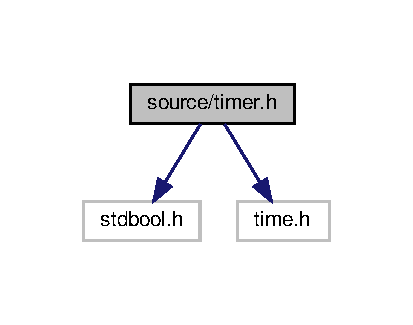
\includegraphics[width=198pt]{timer_8h__incl}
\end{center}
\end{figure}
This graph shows which files directly or indirectly include this file\+:
\nopagebreak
\begin{figure}[H]
\begin{center}
\leavevmode
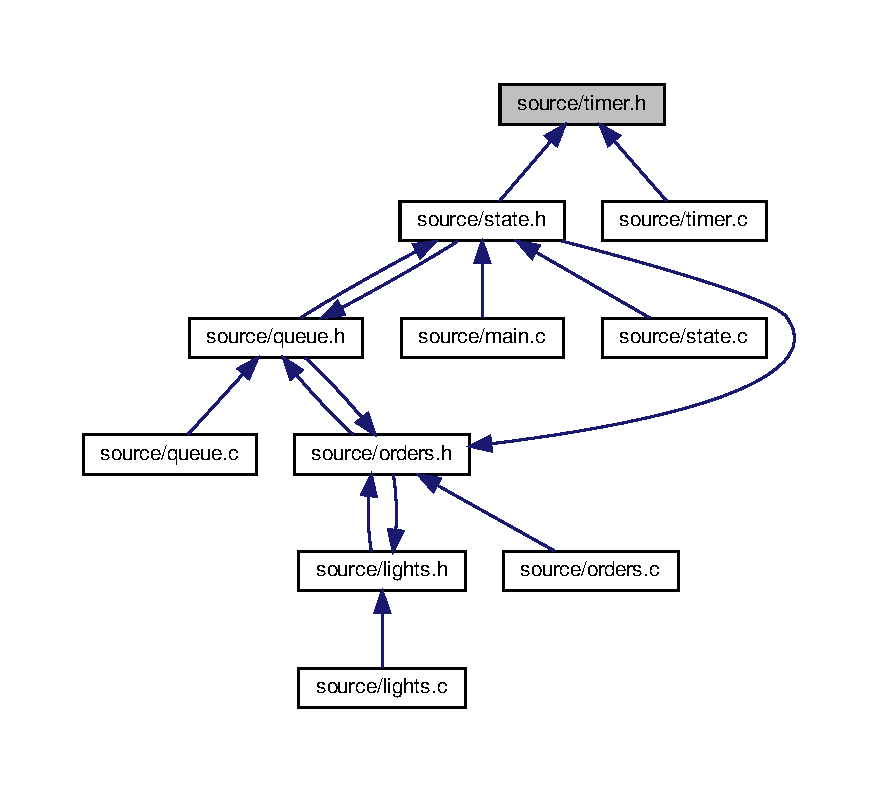
\includegraphics[width=350pt]{timer_8h__dep__incl}
\end{center}
\end{figure}
\subsection*{Functions}
\begin{DoxyCompactItemize}
\item 
\mbox{\Hypertarget{timer_8h_aaedac22c55880495505bf375e0e132c1}\label{timer_8h_aaedac22c55880495505bf375e0e132c1}} 
void \hyperlink{timer_8h_aaedac22c55880495505bf375e0e132c1}{start\+\_\+timer} ()
\begin{DoxyCompactList}\small\item\em Starts timer. Sets a variable equal to the current time, by calling the function time(\+N\+U\+L\+L). \end{DoxyCompactList}\item 
bool \hyperlink{timer_8h_a7ea8455cf4db14c686ca6ac10e8f043b}{timer\+\_\+countdown} ()
\begin{DoxyCompactList}\small\item\em Implementation of the 3 seconds countdown. Checks if the difference between the current time and the start time is higher or lower than the time limit. If higher, it has reached the time limit and returns 1. If lower, returns 0. \end{DoxyCompactList}\end{DoxyCompactItemize}


\subsection{Detailed Description}
Implementation of timer on the elevator door. 



\subsection{Function Documentation}
\mbox{\Hypertarget{timer_8h_a7ea8455cf4db14c686ca6ac10e8f043b}\label{timer_8h_a7ea8455cf4db14c686ca6ac10e8f043b}} 
\index{timer.\+h@{timer.\+h}!timer\+\_\+countdown@{timer\+\_\+countdown}}
\index{timer\+\_\+countdown@{timer\+\_\+countdown}!timer.\+h@{timer.\+h}}
\subsubsection{\texorpdfstring{timer\+\_\+countdown()}{timer\_countdown()}}
{\footnotesize\ttfamily bool timer\+\_\+countdown (\begin{DoxyParamCaption}{ }\end{DoxyParamCaption})}



Implementation of the 3 seconds countdown. Checks if the difference between the current time and the start time is higher or lower than the time limit. If higher, it has reached the time limit and returns 1. If lower, returns 0. 

\begin{DoxyReturn}{Returns}
countdown executed (1). countdown ongoing (0) 
\end{DoxyReturn}


Definition at line 12 of file timer.\+c.


%--- End generated contents ---

% Index
\backmatter
\newpage
\phantomsection
\clearemptydoublepage
\addcontentsline{toc}{chapter}{Index}
\printindex

\end{document}
